
\begin{abstract}
The consistent increase in the world's elder population has been putting a lot of challenges regarding national development, sustainability of families and the ability of health care systems to provide for ageing populations. As wireless sensing technology continues to evolve, devices integrating low-power, low-bandwidth radios and a modest amount of storage, emerge due to considerable reduced costs. Wireless sensors based home monitoring systems provide a safe, sound and secure environment for elder people, enabling them to live in their own home as long as possible. This work introduces the \acf{EMoS}, a \acs{MiXiM} based framework, in which an \acf{AODV} protocol has been implemented together with a modified HORUS system, for tracking and monitoring, in a home environment, elder people or people with special needs. The results obtained from this research demonstrate the feasibility to build a monitoring system for elder care using a simulated environment in which several aspects of the hardware commercially available have been also discussed. 
\end{abstract}


% Note that keywords are not normally used for peerreview papers.
\begin{IEEEkeywords}
Sensor Networks, Elder Care, Routing Protocols, Indoor Location
\end{IEEEkeywords}

% For peer review papers, you can put extra information on the cover
% page as needed:
% \ifCLASSOPTIONpeerreview
% \begin{center} \bfseries EDICS Category: 3-BBND \end{center}
% \fi
%
% For peerreview papers, this IEEEtran command inserts a page break and
% creates the second title. It will be ignored for other modes.
\IEEEpeerreviewmaketitle

\section{Introduction}
% The very first letter is a 2 line initial drop letter followed
% by the rest of the first word in caps.
% 
% form to use if the first word consists of a single letter:
% \IEEEPARstart{A}{demo} file is ....
% 
% form to use if you need the single drop letter followed by
% normal text (unknown if ever used by IEEE):
% \IEEEPARstart{A}{}demo file is ....
% 
% Some journals put the first two words in caps:
% \IEEEPARstart{T}{his demo} file is ....
% 
% Here we have the typical use of a "T" for an initial drop letter
% and "HIS" in caps to complete the first word.
\IEEEPARstart{I}{n} recent years, the increase in life expectancy has been putting a lot of challenges regarding national development, sustainability of families and the ability of health care systems to provide for ageing populations. During recent years the number of people in the world above 60 years has increased from 200 million in 1950 to 670 million, an ageing group that represents already 20\% of the world's total population in developed countries \cite{1}.

\begin{figure}[!htb]
  \centering
  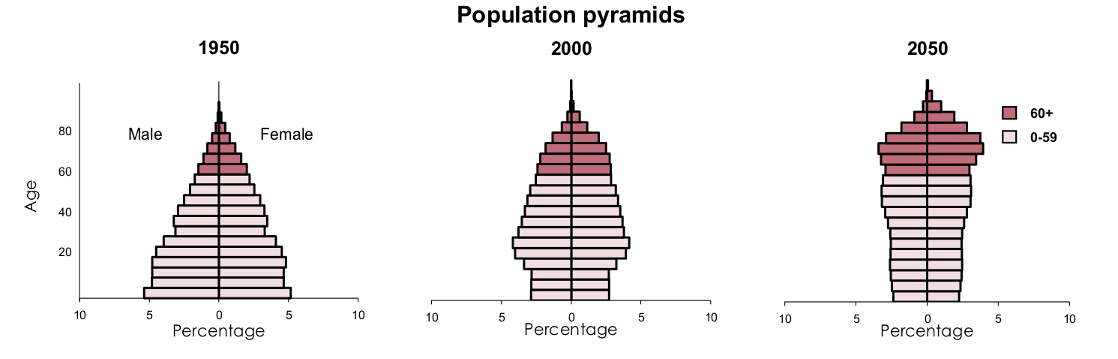
\includegraphics[width=0.50\textwidth]{img/01_demografia_pt.png}
  \caption{Demographic pyramids for Portugal between 1950 and 2050\cite{1}.}
  \label{fig:1:demog_pt}
\end{figure}
 
With the relocation of young people to the suburbs and the low birth rate, the number of elder people who live home alone is increasing. This  situation creates a huge anxiety in all the people involved, resulting many times in early institutionalization in caring homes or other elder care facilities. Also people with physical or mental disabilities present identical caring needs. For example, people with mild mental retardation usually achieve sufficient social and vocational capabilities for minimal self-support. Problems with these people occur because they have trouble getting in/out of bed on time. The lack of overview and planning skills to see that they have to go to bed on time in order to be able to go to work on time the next day.\\
Creating a system able to monitor people in this situation would allow  specialized professionals to dedicate their work to other types of scenarios where a larger dependency would exist freeing costly and rare resources. As wireless sensor technology continues to evolve, devices integrating low-power, low-bandwidth radios and a modest amount of storage emerge with a considerable low cost. With a vast number of existing sensors, ubiquitous applications can emerge as a low cost alternative with huge added value for monitoring people in a home environment, providing a huge symbiosis between man and machine.\\
This work suggests the development of a system, where one or more persons, carrying a node with wireless capabilities, move around an environment where other wireless sensors exist. The system should be able to identify each individual and allow for communication with a central base station in a bidirectional way.\\
The rest of this paper is organized in the following manner.\\In Chapter 2 a research about the state-of-the-art solutions is made with reference to systems the employ video, wearable sensors and home appliances sensors to monitor people in a home environment.\\
Chapter 3 talks about the related work, focusing on elder people needs in healthcare, through a study where interviews were made to \acp{CM}. This chapter also refers to the usage of wireless sensors for tracking and compares routing protocols.\\
In chapter 4 the work environment for the simulation is presented together with the difficulties in getting a simulator that can achieve a high degree of accuracy while simulating movement, obstacles and wireless sensor networks.\\
In chapter 5 the \acf{EMoS} is presented together with an evaluation of real hardware options commercially available, capable of implementing the system in real conditions.\\
Chapter 6 discusses and analyses results from the simulation.\\
Conclusions and future work are presented in chapter 7.




% \hfill initials

% \hfill Month Day, Year

...



% An example of a floating figure using the graphicx package.
% Note that \label must occur AFTER (or within) \caption.
% For figures, \caption should occur after the \includegraphics.
% Note that IEEEtran v1.7 and later has special internal code that
% is designed to preserve the operation of \label within \caption
% even when the captionsoff option is in effect. However, because
% of issues like this, it may be the safest practice to put all your
% \label just after \caption rather than within \caption{}.
%
% Reminder: the "draftcls" or "draftclsnofoot", not "draft", class
% option should be used if it is desired that the figures are to be
% displayed while in draft mode.
%
%\begin{figure}[!t]
%\centering
%\includegraphics[width=2.5in]{myfigure}
% where an .eps filename suffix will be assumed under latex, 
% and a .pdf suffix will be assumed for pdflatex; or what has been declared
% via \DeclareGraphicsExtensions.
%\caption{Simulation Results}
%\label{fig_sim}
%\end{figure}

% Note that IEEE typically puts floats only at the top, even when this
% results in a large percentage of a column being occupied by floats.


% An example of a double column floating figure using two subfigures.
% (The subfig.sty package must be loaded for this to work.)
% The subfigure \label commands are set within each subfloat command, the
% \label for the overall figure must come after \caption.
% \hfil must be used as a separator to get equal spacing.
% The subfigure.sty package works much the same way, except \subfigure is
% used instead of \subfloat.
%
%\begin{figure*}[!t]
%\centerline{\subfloat[Case I]\includegraphics[width=2.5in]{subfigcase1}%
%\label{fig_first_case}}
%\hfil
%\subfloat[Case II]{\includegraphics[width=2.5in]{subfigcase2}%
%\label{fig_second_case}}}
%\caption{Simulation results}
%\label{fig_sim}
%\end{figure*}
%
% Note that often IEEE papers with subfigures do not employ subfigure
% captions (using the optional argument to \subfloat), but instead will
% reference/describe all of them (a), (b), etc., within the main caption.


% An example of a floating table. Note that, for IEEE style tables, the 
% \caption command should come BEFORE the table. Table text will default to
% \footnotesize as IEEE normally uses this smaller font for tables.
% The \label must come after \caption as always.
%
%\begin{table}[!t]
%% increase table row spacing, adjust to taste
%\renewcommand{\arraystretch}{1.3}
% if using array.sty, it might be a good idea to tweak the value of
% \extrarowheight as needed to properly center the text within the cells
%\caption{An Example of a Table}
%\label{table_example}
%\centering
%% Some packages, such as MDW tools, offer better commands for making tables
%% than the plain LaTeX2e tabular which is used here.
%\begin{tabular}{|c||c|}
%\hline
%One & Two\\
%\hline
%Three & Four\\
%\hline
%\end{tabular}
%\end{table}


% Note that IEEE does not put floats in the very first column - or typically
% anywhere on the first page for that matter. Also, in-text middle ("here")
% positioning is not used. Most IEEE journals use top floats exclusively.
% Note that, LaTeX2e, unlike IEEE journals, places footnotes above bottom
% floats. This can be corrected via the \fnbelowfloat command of the
% stfloats package.